\documentclass[aspectratio=169, 10pt]{beamer}

% ---------- Tema y colores ----------
\usetheme{default}
\usecolortheme{default}
\setbeamertemplate{navigation symbols}{}
\setbeamertemplate{footline}[frame number]
\setbeamertemplate{frametitle continuation}{}

\definecolor{StanfordRed}{RGB}{140,21,21}
\definecolor{StanfordGray}{RGB}{77,77,77}
\definecolor{LightGray}{RGB}{240,240,240}
\definecolor{AccentBlue}{RGB}{0,84,166}
\definecolor{AccentGreen}{RGB}{0,130,100}
\definecolor{UCMBlue}{RGB}{4, 171, 226}
\definecolor{UCMNavy}{RGB}{20, 65, 134}

% Alias de la paleta antigua: las figuras TikZ de esta clase siguen
% usando mitblue/mitgray, que ahora apuntan a los colores UCM.
\definecolor{mitblue}{RGB}{20, 65, 134}
\definecolor{mitgray}{RGB}{169, 169, 169}
\definecolor{backgroundblue}{HTML}{D7EAF3}
\definecolor{catyellow}{HTML}{FCDA76}
\definecolor{catstripe}{HTML}{F9B74C}
\definecolor{yarnred}{HTML}{E26B6B}
\definecolor{bowlblue}{HTML}{66A3D4}
\definecolor{bboxblue}{HTML}{5E69B1}
\definecolor{bboxred}{HTML}{D9534F}
\definecolor{bboxgreen}{HTML}{008000}

\setbeamercolor{frametitle}{fg=white, bg=UCMBlue}
\setbeamercolor{title}{fg=white}
\setbeamercolor{author}{fg=white}
\setbeamercolor{institute}{fg=white!80}
\setbeamercolor{structure}{fg=UCMBlue}
\setbeamercolor{block title}{bg=UCMBlue!15!white, fg=UCMBlue}
\setbeamercolor{block body}{bg=LightGray}
\setbeamercolor{block title alerted}{bg=StanfordRed!15!white, fg=StanfordRed}
\setbeamercolor{block body alerted}{bg=LightGray}
\setbeamercolor{block title example}{bg=AccentGreen!15!white, fg=AccentGreen}
\setbeamercolor{block body example}{bg=LightGray}
\setbeamercolor{alerted text}{fg=UCMBlue}
\setbeamercolor{example text}{fg=UCMBlue}

\setbeamerfont{frametitle}{series=\bfseries, size=\large}
\setbeamerfont{title}{series=\bfseries, size=\LARGE}
\setbeamerfont{block title}{series=\bfseries}

% ---------- Paquetes ----------
\usepackage[utf8]{inputenc}
\usepackage[T1]{fontenc}
\usepackage[provide=*,spanish]{babel}
\usepackage{amsmath, amssymb, bm}
\usepackage{graphicx}
\usepackage{tikz}
\usepackage{pgfplots}
\pgfplotsset{compat=1.18}
\usetikzlibrary{arrows, arrows.meta, shapes, shapes.geometric, positioning,
	fit, calc, matrix, chains, mindmap, decorations.pathreplacing,
	backgrounds, shadows, patterns}
\usepackage{booktabs}
\usepackage{xcolor}
\usepackage{multicol}
\usepackage{tcolorbox}
\tcbuselibrary{skins, breakable}
\usepackage{tikzlings}


% ---------- Comandos útiles ----------
\providecommand{\R}{\mathbb{R}}
\providecommand{\E}{\mathbb{E}}
\providecommand{\IoU}{\operatorname{IoU}}

\newcommand{\formula}[1]{%
	\begin{tcolorbox}[colback=UCMBlue!8, colframe=UCMBlue, arc=4pt,
		boxsep=2pt, left=6pt, right=6pt, top=3pt, bottom=3pt]
		#1
	\end{tcolorbox}
}

% ---------- Portada ----------
\title{\textbf{Detecci\'on de Objetos}}
\subtitle{Cajas ancla, SSD y la familia R-CNN}
\author{Sergio Hern\'andez, PhD\\ shernandez@ucm.cl}
\institute{
	\begin{tikzpicture}[scale=0.42, every node/.style={transform shape}]
		\foreach \i/\y in {1/0,2/1,3/2}{\node[circle,draw=white,fill=white!20,minimum size=4mm] (i\i) at (0,\y){};}
		\foreach \i/\y in {1/-0.5,2/0.5,3/1.5,4/2.5}{\node[circle,draw=white,fill=white!35,minimum size=4mm] (h\i) at (2,\y){};}
		\foreach \i/\y in {1/0.5,2/1.5}{\node[circle,draw=white,fill=white!50,minimum size=4mm] (o\i) at (4,\y){};}
		\foreach \a in {1,2,3}\foreach \b in {1,2,3,4}{\draw[white,opacity=0.5] (i\a)--(h\b);}
		\foreach \a in {1,2,3,4}\foreach \b in {1,2}{\draw[white,opacity=0.5] (h\a)--(o\b);}
	\end{tikzpicture}
	\\ \textbf{Mag\'ister en Data Science --- Universidad Cat\'olica del Maule}}
\date{}


\begin{document}
% --- Título ---
{
	\setbeamertemplate{background}{
		
\begin{tikzpicture}[remember picture, overlay]
			\fill[UCMBlue] (current page.south west) rectangle (current page.north east);
			\fill[UCMBlue!70!black, opacity=0.5]
			(current page.south west) -- ++(0,3) -- ++(18,0) -- cycle;
			\foreach \i in {1,...,40}{
				\fill[white, opacity=0.04]
				({random()*17}, {random()*10}) circle ({random()*0.3});
			}
		\end{tikzpicture}
	}
	\begin{frame}[plain]
		\vspace{1.2cm}
		\titlepage
		\begin{tikzpicture}[remember picture, overlay]
			\node[white, opacity=0.15, font=\fontsize{80}{80}\selectfont]
			at (current page.east) [xshift=-2cm] {$\boxdot$};
		\end{tikzpicture}
	\end{frame}
}

% =================================================================
% SECCIÓN 1: INTRODUCCIÓN
\section{Introducci\'on}

\begin{frame}{De la Clasificación a la Detección}
	\begin{columns}[T]
		\begin{column}{0.5\textwidth}
			\begin{block}{Clasificación}
				Una imagen $\rightarrow$ \textbf{una} etiqueta. Asume que hay un único objeto dominante.
			\end{block}
			\begin{block}{Detección de objetos}
				Una imagen $\rightarrow$ un número \textbf{variable} de objetos, cada uno con:
				\begin{itemize}
					\item su \textbf{categoría} $y_c \in \{1,\ldots,q\}$,
					\item su \textbf{ubicación}: una caja delimitadora (\textit{bounding box}) $y_l \in \R^4$.
				\end{itemize}
			\end{block}
			\small Aplicaciones: vehículos autónomos, vigilancia, imágenes médicas, conteo de objetos.
		\end{column}
		\begin{column}{0.5\textwidth}
			\begin{center}
				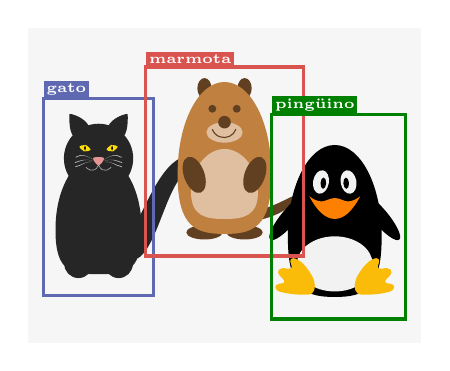
\begin{tikzpicture}
					\node[rectangle, fill=mitgray!10, minimum width=5cm, minimum height=4cm] at (2.2, 1.7) {};
					\cat[xshift=0.6cm,yshift=0.4cm];
					\marmot[xshift=2.2cm,yshift=0.9cm];
					\penguin[xshift=3.6cm,yshift=0.1cm];
					\draw [bboxblue, very thick] (-0.1,0.3) rectangle (1.3,2.8);
					\draw [bboxred, very thick] (1.2,0.8) rectangle (3.2,3.2);
					\draw [bboxgreen, very thick] (2.8,0.0) rectangle (4.5,2.6);
					\node[fill=bboxblue, text=white, font=\tiny\bfseries, anchor=south west, inner sep=1pt] at (-0.1,2.8) {gato};
					\node[fill=bboxred, text=white, font=\tiny\bfseries, anchor=south west, inner sep=1pt] at (1.2,3.2) {marmota};
					\node[fill=bboxgreen, text=white, font=\tiny\bfseries, anchor=south west, inner sep=1pt] at (2.8,2.6) {pingüino};
				\end{tikzpicture}
			\end{center}
		\end{column}
	\end{columns}
\end{frame}

\begin{frame}{Representación de una Caja Delimitadora}
	\begin{columns}[T]
		\begin{column}{0.52\textwidth}
			Una caja rectangular se describe con 4 números. Hay dos convenciones habituales:
			\begin{block}{Esquinas $(x_1, y_1, x_2, y_2)$}
				Esquina superior izquierda y esquina inferior derecha.
			\end{block}
			\begin{block}{Centro $(c_x, c_y, w, h)$}
				Centro de la caja, ancho y alto.
			\end{block}
			\formula{\vspace{-0.3cm}
				\begin{align*}
					c_x &= \tfrac{x_1+x_2}{2}, & c_y &= \tfrac{y_1+y_2}{2},\\
					w &= x_2-x_1, & h &= y_2-y_1
				\end{align*}}
			\small En imágenes el origen está en la esquina \textbf{superior izquierda} y el eje $y$ crece hacia abajo.
		\end{column}
		\begin{column}{0.46\textwidth}
			\begin{center}
				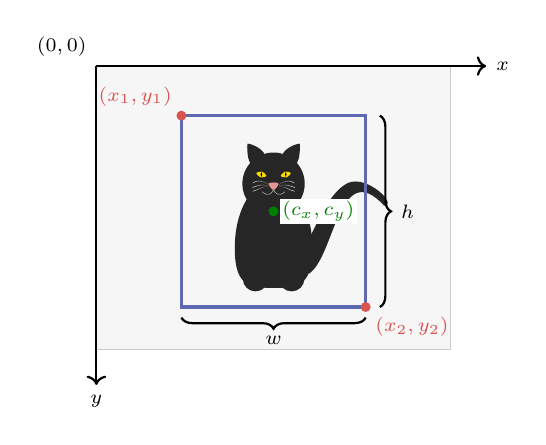
\begin{tikzpicture}[yscale=-1, scale=0.9]
					% imagen
					\draw[mitgray!60, fill=mitgray!10] (0,0) rectangle (5,4);
					\draw[->, thick] (0,0) -- (5.5,0) node[right, font=\scriptsize] {$x$};
					\draw[->, thick] (0,0) -- (0,4.5) node[below, font=\scriptsize] {$y$};
					\node[font=\scriptsize, anchor=south east] at (0,0) {$(0,0)$};
					% objeto
					\begin{scope}[yscale=-1, yshift=-3.3cm]
						\cat[xshift=2.5cm,yshift=0cm];
					\end{scope}
					\draw[bboxblue, very thick] (1.2,0.7) rectangle (3.8,3.4);
					\fill[bboxred] (1.2,0.7) circle (2pt) node[above left, font=\scriptsize] {$(x_1,y_1)$};
					\fill[bboxred] (3.8,3.4) circle (2pt) node[below right, font=\scriptsize] {$(x_2,y_2)$};
					\fill[bboxgreen] (2.5,2.05) circle (2pt) node[right, font=\scriptsize, text=bboxgreen, fill=white, inner sep=1pt, xshift=2pt] {$(c_x,c_y)$};
					\draw[decorate, decoration={brace, amplitude=4pt, mirror}, thick] (1.2,3.55) -- (3.8,3.55) node[midway, below=3pt, font=\scriptsize] {$w$};
					\draw[decorate, decoration={brace, amplitude=4pt}, thick] (4.0,0.7) -- (4.0,3.4) node[midway, right=4pt, font=\scriptsize] {$h$};
				\end{tikzpicture}
			\end{center}
		\end{column}
	\end{columns}
\end{frame}

\begin{frame}{¿Cómo proponer las cajas candidatas?}
	\begin{block}{El problema central}
		No sabemos \textbf{cuántos} objetos hay ni \textbf{dónde} están. El modelo debe muestrear muchas regiones candidatas, decidir si contienen un objeto y ajustar sus bordes.
	\end{block}
	\vspace{0.2cm}
	\begin{columns}[T]
		\begin{column}{0.5\textwidth}
			\begin{exampleblock}{Una etapa (\textit{one-stage})}
				Se colocan \textbf{cajas ancla} fijas sobre la imagen y una sola red predice clase y ajuste para cada ancla.
				\begin{itemize}
					\item SSD, YOLO, RetinaNet.
					\item Rápidos, adecuados para tiempo real.
				\end{itemize}
			\end{exampleblock}
		\end{column}
		\begin{column}{0.5\textwidth}
			\begin{alertblock}{Dos etapas (\textit{two-stage})}
				Primero se generan \textbf{propuestas de región}; luego una segunda red las clasifica y refina.
				\begin{itemize}
					\item R-CNN, Fast R-CNN, Faster R-CNN, Mask R-CNN.
					\item Más precisos, más costosos.
				\end{itemize}
			\end{alertblock}
		\end{column}
	\end{columns}
	\vspace{0.2cm}
	\centering Ambas familias comparten las mismas piezas: \textbf{anclas, IoU, desplazamientos y NMS}.
\end{frame}

% =================================================================
% SECCIÓN 2: CAJAS ANCLA
\section{Cajas ancla}

\begin{frame}{Cajas Ancla (\textit{Anchor Boxes})}
	\begin{columns}[T]
		\begin{column}{0.55\textwidth}
			Para una imagen de ancho $w$ y alto $h$, centramos en cada píxel cajas de distintas formas, definidas por una \textbf{escala} $s \in (0,1]$ y una \textbf{razón de aspecto} $r>0$:
			\formula{\[
				\text{ancho} = w\, s\sqrt{r}, \qquad \text{alto} = \frac{h\, s}{\sqrt{r}}
			\]}
			Con escalas $s_1,\ldots,s_n$ y razones $r_1,\ldots,r_m$ no se usan las $nm$ combinaciones, sólo las que contienen $s_1$ o $r_1$:
			\[
			(s_1,r_1),\ldots,(s_1,r_m),\ (s_2,r_1),\ldots,(s_n,r_1)
			\]
			$\Rightarrow$ \textbf{$n+m-1$ anclas por píxel} y $wh(n+m-1)$ en total.
		\end{column}
		\begin{column}{0.43\textwidth}
			\begin{center}
				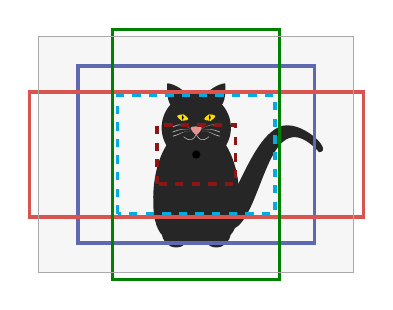
\begin{tikzpicture}
					\fill[mitgray!10] (0,0) rectangle (4,3);
					\cat[xshift=2cm,yshift=0.2cm];
					\begin{scope}
						% s=0.75, r=1,2,0.5
						\draw[bboxblue, very thick] (0.5,0.375) rectangle (3.5,2.625);
						\draw[bboxred, very thick] (-0.12,0.705) rectangle (4.12,2.295);
						\draw[bboxgreen, very thick] (0.94,-0.09) rectangle (3.06,3.09);
						% s=0.5, 0.25, r=1
						\draw[UCMBlue, very thick, dashed] (1,0.75) rectangle (3,2.25);
						\draw[StanfordRed, very thick, dashed] (1.5,1.125) rectangle (2.5,1.875);
					\end{scope}
					\draw[mitgray] (0,0) rectangle (4,3);
					\fill (2,1.5) circle (1.5pt);
				\end{tikzpicture}

				\vspace{0.2cm}
				\scriptsize
				\begin{tabular}{ll}
					\textcolor{bboxblue}{\rule{8pt}{2pt}} $s=0.75, r=1$ & \textcolor{UCMBlue}{\rule{8pt}{2pt}} $s=0.5, r=1$\\
					\textcolor{bboxred}{\rule{8pt}{2pt}} $s=0.75, r=2$ & \textcolor{StanfordRed}{\rule{8pt}{2pt}} $s=0.25, r=1$\\
					\textcolor{bboxgreen}{\rule{8pt}{2pt}} $s=0.75, r=0.5$ &
				\end{tabular}

				\vspace{0.1cm}
				$n=3,\ m=3 \Rightarrow 5$ anclas por píxel.
			\end{center}
		\end{column}
	\end{columns}
\end{frame}

\begin{frame}{Intersección sobre Unión (IoU)}
	\begin{columns}[c]
		\begin{column}{0.55\textwidth}
			Para medir qué tan bien un ancla cubre un objeto usamos el \textbf{índice de Jaccard}:
			\formula{\[
				J(\mathcal{A},\mathcal{B}) = \IoU(\mathcal{A},\mathcal{B}) = \frac{|\mathcal{A}\cap\mathcal{B}|}{|\mathcal{A}\cup\mathcal{B}|} \in [0,1]
			\]}
			\begin{itemize}
				\item $\IoU=1$: cajas idénticas; $\IoU=0$: sin solapamiento.
				\item Para cajas en formato esquinas, la intersección va de
				$\big(\max(x_1,x_1'), \max(y_1,y_1')\big)$ a $\big(\min(x_2,x_2'), \min(y_2,y_2')\big)$.
				\item Se usa en tres lugares: \textbf{asignar} etiquetas a las anclas, \textbf{suprimir} predicciones redundantes y \textbf{evaluar} al detector.
			\end{itemize}
		\end{column}
		\begin{column}{0.43\textwidth}
			\begin{center}
				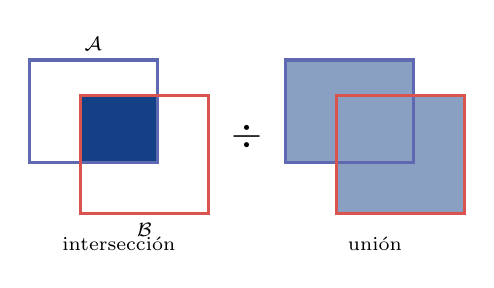
\begin{tikzpicture}[scale=0.65]
					\begin{scope}
						\fill[mitblue] (1,0.5) rectangle (2.5,1.8);
						\draw[bboxblue, very thick] (0,0.5) rectangle (2.5,2.5);
						\draw[bboxred, very thick] (1,-0.5) rectangle (3.5,1.8);
						\node[font=\scriptsize, anchor=south] at (1.25,2.5) {$\mathcal{A}$};
						\node[font=\scriptsize, anchor=north] at (2.25,-0.5) {$\mathcal{B}$};
					\end{scope}
					\node[font=\Large] at (4.25,1) {$\div$};
					\begin{scope}[xshift=5cm]
						\fill[mitblue!50] (0,0.5) -- (0,2.5) -- (2.5,2.5) -- (2.5,1.8) -- (3.5,1.8) -- (3.5,-0.5) -- (1,-0.5) -- (1,0.5) -- cycle;
						\draw[bboxblue, very thick] (0,0.5) rectangle (2.5,2.5);
						\draw[bboxred, very thick] (1,-0.5) rectangle (3.5,1.8);
					\end{scope}
					\node[font=\scriptsize] at (1.75,-1.1) {intersección};
					\node[font=\scriptsize] at (6.75,-1.1) {unión};
				\end{tikzpicture}
			\end{center}
		\end{column}
	\end{columns}
\end{frame}

\begin{frame}{Asignar Cajas Reales a las Anclas}
	\begin{columns}[T]
		\begin{column}{0.55\textwidth}
			Sean $A_1,\ldots,A_{n_a}$ las anclas y $B_1,\ldots,B_{n_b}$ las cajas reales ($n_a \geq n_b$). Construimos la matriz $\mathbf{X}\in\R^{n_a\times n_b}$ con $x_{ij}=\IoU(A_i,B_j)$.
			\begin{enumerate}
				\item Buscar el \textbf{mayor} elemento $x_{ij}$ de $\mathbf{X}$ y asignar $B_j$ al ancla $A_i$.
				\item Descartar la fila $i$ y la columna $j$.
				\item Repetir hasta asignar las $n_b$ cajas reales.
				\item Para las anclas restantes: asignar la caja $B_j$ de mayor IoU \textbf{sólo si} supera un umbral (p.ej. $0.5$).
			\end{enumerate}
			\small Las anclas sin caja asignada se etiquetan como \textbf{fondo} (clase $0$).
		\end{column}
		\begin{column}{0.43\textwidth}
			\begin{center}
				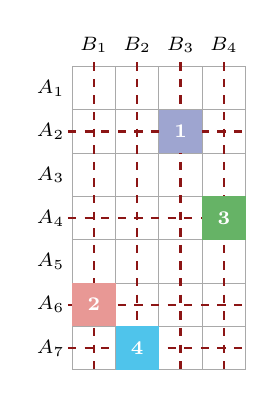
\begin{tikzpicture}[scale=0.55]
					\foreach \j in {1,...,4} \node[font=\scriptsize] at (\j-0.5, 0.5) {$B_\j$};
					\foreach \i in {1,...,7} \node[font=\scriptsize] at (-0.5, -\i+0.5) {$A_\i$};
					% grilla
					\draw[mitgray] (0,-7) grid (4,0);
					% filas y columnas descartadas
					\foreach \y in {-1.5,-3.5,-5.5,-6.5} \draw[StanfordRed, dashed, thick] (-0.1,\y) -- (4.1,\y);
					\foreach \x in {0.5,1.5,2.5,3.5} \draw[StanfordRed, dashed, thick] (\x,0.1) -- (\x,-7.1);
					% celdas asignadas (orden 1..4)
					\fill[bboxblue!60] (2,-2) rectangle (3,-1);   \node[white,font=\scriptsize\bfseries] at (2.5,-1.5) {1};
					\fill[bboxred!60] (0,-6) rectangle (1,-5);    \node[white,font=\scriptsize\bfseries] at (0.5,-5.5) {2};
					\fill[bboxgreen!60] (3,-4) rectangle (4,-3);  \node[white,font=\scriptsize\bfseries] at (3.5,-3.5) {3};
					\fill[UCMBlue!70] (1,-7) rectangle (2,-6);    \node[white,font=\scriptsize\bfseries] at (1.5,-6.5) {4};
				\end{tikzpicture}

				\scriptsize Orden en que se toman los máximos de $\mathbf{X}$; en cada paso se tachan su fila y su columna.
			\end{center}
		\end{column}
	\end{columns}
\end{frame}

\begin{frame}{Etiquetas: Clases y Desplazamientos}
	Cada ancla $A$ recibe como objetivo la \textbf{clase} de su caja asignada $B$ y un \textbf{desplazamiento} (\textit{offset}) que indica cómo transformar $A$ en $B$.

	\vspace{0.2cm}
	Con $A=(x_a,y_a,w_a,h_a)$ y $B=(x_b,y_b,w_b,h_b)$ en formato centro:
	\formula{\[
		\left(
		\frac{\frac{x_b-x_a}{w_a}-\mu_x}{\sigma_x},\;
		\frac{\frac{y_b-y_a}{h_a}-\mu_y}{\sigma_y},\;
		\frac{\log\frac{w_b}{w_a}-\mu_w}{\sigma_w},\;
		\frac{\log\frac{h_b}{h_a}-\mu_h}{\sigma_h}
		\right)
		\]}
	con valores por defecto $\mu_x=\mu_y=\mu_w=\mu_h=0$, $\sigma_x=\sigma_y=0.1$, $\sigma_w=\sigma_h=0.2$.

	\begin{itemize}
		\item Las traslaciones se normalizan por el tamaño del ancla y las escalas se toman en \textbf{logaritmo}: el objetivo queda en un rango similar para cajas grandes y pequeñas.
		\item Las anclas de \textbf{fondo} no tienen desplazamiento válido: se \textbf{enmascaran} en la pérdida de localización.
	\end{itemize}
\end{frame}

\begin{frame}{Supresión de No-Máximos (NMS)}
	\begin{columns}[T]
		\begin{column}{0.55\textwidth}
			En predicción, muchas anclas cercanas detectan el mismo objeto. NMS conserva sólo la mejor:
			\begin{enumerate}
				\item Ordenar las cajas predichas $L$ por confianza (probabilidad de la clase predicha, sin fondo).
				\item Tomar la de mayor confianza $B_1$ como \textbf{base} y eliminar de $L$ toda caja con $\IoU(B_1,\cdot) > \epsilon$.
				\item Repetir con la siguiente caja de mayor confianza que siga en $L$.
				\item Terminar cuando todas las cajas de $L$ hayan sido base.
			\end{enumerate}
			\small Resultado: ningún par de cajas retenidas tiene IoU mayor que $\epsilon$.
		\end{column}
		\begin{column}{0.43\textwidth}
			\begin{center}
				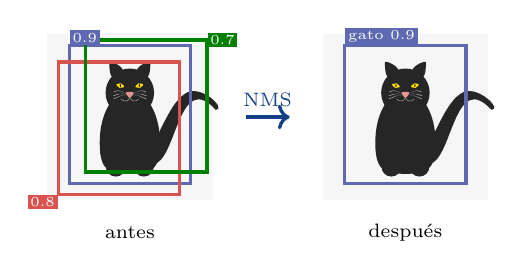
\begin{tikzpicture}[scale=0.7]
					\begin{scope}
						\fill[mitgray!10] (0,0) rectangle (3,3);
						\cat[xshift=1.5cm,yshift=0.3cm];
						\draw[bboxblue, very thick] (0.4,0.3) rectangle (2.6,2.8);
						\draw[bboxred, very thick] (0.2,0.1) rectangle (2.4,2.5);
						\draw[bboxgreen, very thick] (0.7,0.5) rectangle (2.9,2.9);
						\node[fill=bboxblue, text=white, font=\tiny, inner sep=1pt, anchor=south west] at (0.4,2.8) {0.9};
						\node[fill=bboxred, text=white, font=\tiny, inner sep=1pt, anchor=north east] at (0.2,0.1) {0.8};
						\node[fill=bboxgreen, text=white, font=\tiny, inner sep=1pt, anchor=west] at (2.9,2.9) {0.7};
						\node[font=\scriptsize] at (1.5,-0.6) {antes};
					\end{scope}
					\draw[->, very thick, mitblue] (3.6,1.5) -- (4.4,1.5) node[midway, above, font=\scriptsize] {NMS};
					\begin{scope}[xshift=5cm]
						\fill[mitgray!10] (0,0) rectangle (3,3);
						\cat[xshift=1.5cm,yshift=0.3cm];
						\draw[bboxblue, very thick] (0.4,0.3) rectangle (2.6,2.8);
						\node[fill=bboxblue, text=white, font=\tiny, inner sep=1pt, anchor=south west] at (0.4,2.8) {gato 0.9};
						\node[font=\scriptsize] at (1.5,-0.6) {después};
					\end{scope}
				\end{tikzpicture}
			\end{center}
		\end{column}
	\end{columns}
\end{frame}

% =================================================================
% SECCIÓN 3: DETECCIÓN MULTIESCALA
\section{Detecci\'on multiescala}

\begin{frame}{Detección Multiescala}
	\begin{block}{Demasiadas anclas}
		Una imagen de $561\times728$ con 5 anclas por píxel genera más de \textbf{2 millones} de cajas a clasificar.
	\end{block}
	\textbf{Idea:} generar anclas sobre \textbf{mapas de características} de distintos tamaños, en lugar de sobre cada píxel.
	\begin{itemize}
		\item Mapas grandes (muchas celdas) $\rightarrow$ anclas \textbf{pequeñas y densas}: objetos pequeños.
		\item Mapas pequeños (pocas celdas) $\rightarrow$ anclas \textbf{grandes y escasas}: objetos grandes.
	\end{itemize}
	\begin{center}
		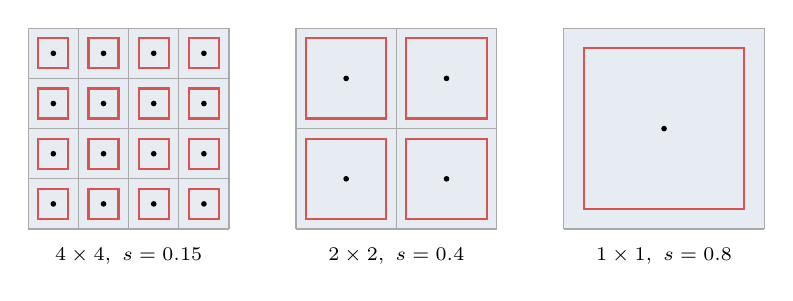
\begin{tikzpicture}[scale=0.85]
			\foreach \n/\s/\x/\lab in {4/0.15/0/{$4\times4,\ s=0.15$}, 2/0.4/4/{$2\times2,\ s=0.4$}, 1/0.8/8/{$1\times1,\ s=0.8$}}{
				\begin{scope}[xshift=\x cm]
					\fill[mitblue!10] (0,0) rectangle (3,3);
					\pgfmathsetmacro\c{3/\n}
					\draw[mitgray, step=\c] (0,0) grid (3,3);
					\pgfmathsetmacro\half{1.5*\s}
					\pgfmathtruncatemacro\nm{\n-1}
					\foreach \i in {0,...,\nm}\foreach \j in {0,...,\nm}{
						\pgfmathsetmacro\cx{(\i+0.5)*\c}
						\pgfmathsetmacro\cy{(\j+0.5)*\c}
						\fill (\cx,\cy) circle (1.2pt);
						\draw[bboxred, thick] ({\cx-\half},{\cy-\half}) rectangle ({\cx+\half},{\cy+\half});
					}
					\node[font=\scriptsize] at (1.5,-0.4) {\lab};
				\end{scope}
			}
		\end{tikzpicture}
	\end{center}
	\small Las unidades más cercanas a la salida tienen un \textbf{campo receptivo} mayor, por lo que \textbf{pueden} detectar objetos más grandes.
\end{frame}

% =================================================================
% SECCIÓN 4: SSD
\section{SSD}

\begin{frame}{Single Shot Multibox Detection (SSD)}
	SSD (Liu et al., 2016) es un detector de \textbf{una etapa}: una red base seguida de bloques que reducen el mapa de características a la mitad. \textbf{Cada escala} genera anclas y predice clases y desplazamientos.
	\begin{center}
		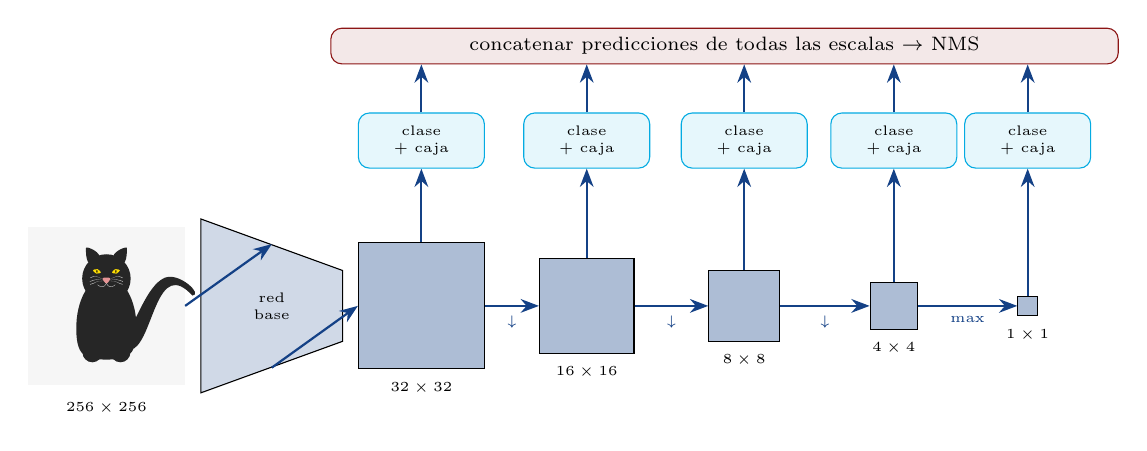
\begin{tikzpicture}[
			fmap/.style={draw=black, fill=mitblue, fill opacity=0.35, text opacity=1},
			pred/.style={draw=UCMBlue, fill=UCMBlue!10, rounded corners, font=\tiny, align=center, minimum width=1.6cm, minimum height=0.7cm},
			arr/.style={-{Stealth}, thick, mitblue}]
			% entrada
			\fill[mitgray!10] (-2.2,-1) rectangle (-0.2,1);
			\cat[xshift=-1.2cm,yshift=-0.8cm,scale=0.7];
			\node[font=\tiny] at (-1.2,-1.3) {$256\times256$};
			% red base
			\node[draw, fill=mitblue!20, trapezium, trapezium left angle=70, trapezium right angle=70, shape border rotate=270, minimum height=1.8cm, font=\tiny, align=center, text width=0.9cm] (base) at (0.9,0) {red\\base};
			\draw[arr] (-0.2,0) -- (base.north);
			% mapas
			\foreach \k/\sz/\x/\lab in {1/1.6/2.8/{32}, 2/1.2/4.9/{16}, 3/0.9/6.9/{8}, 4/0.6/8.8/{4}, 5/0.25/10.5/{1}}{
				\node[fmap, minimum width=\sz cm, minimum height=\sz cm] (m\k) at (\x,0) {};
				\node[font=\tiny, below=1pt] at (m\k.south) {$\lab\times\lab$};
				\node[pred] (p\k) at (\x,2.1) {clase\\+ caja};
				\draw[arr] (m\k.north) -- (p\k.south);
			}
			\draw[arr] (base.south) -- (m1.west);
			\draw[arr] (m1.east) -- node[below, font=\tiny]{$\downarrow$} (m2.west);
			\draw[arr] (m2.east) -- node[below, font=\tiny]{$\downarrow$} (m3.west);
			\draw[arr] (m3.east) -- node[below, font=\tiny]{$\downarrow$} (m4.west);
			\draw[arr] (m4.east) -- node[below, font=\tiny]{max} (m5.west);
			% concatenación
			\node[draw=StanfordRed, fill=StanfordRed!10, rounded corners, font=\scriptsize, minimum width=10cm] (cat) at (6.65,3.3) {concatenar predicciones de todas las escalas $\rightarrow$ NMS};
			\foreach \k in {1,...,5} \draw[arr] (p\k.north) -- (p\k.north |- cat.south);
		\end{tikzpicture}
	\end{center}
	\small $\downarrow$: bloque de reducción ($2\times$[conv $3\times3$ + BatchNorm + ReLU] + max-pool $2\times2$). El último bloque usa max-pooling global.
\end{frame}

\begin{frame}{SSD: Capas de Predicción}
	Sea $q$ el número de clases y $a$ el número de anclas por celda de un mapa $h\times w$.
	\begin{columns}[T]
		\begin{column}{0.5\textwidth}
			\begin{block}{Predicción de clase}
				Convolución $3\times3$ con padding $1$ (conserva $h\times w$) y
				\begin{center}\textcolor{UCMBlue}{\boldmath$a(q+1)$} canales de salida\end{center}
				El canal $i(q+1)+j$ es el puntaje de la clase $j$ ($j=0$: fondo) para el ancla $i$.
			\end{block}
		\end{column}
		\begin{column}{0.5\textwidth}
			\begin{block}{Predicción de caja}
				Misma estructura, pero con
				\begin{center}\textcolor{UCMBlue}{\boldmath$4a$} canales de salida\end{center}
				los 4 desplazamientos de cada ancla.
			\end{block}
		\end{column}
	\end{columns}
	\vspace{0.2cm}
	Las salidas de cada escala tienen formas distintas: se \textbf{aplanan} y \textbf{concatenan}. Con entrada $256\times256$, escalas $32,16,8,4,1$ y $a=4$:
	\[
	4\,(32^2+16^2+8^2+4^2+1^2) = 5\,444 \text{ anclas}.
	\]
	\small El uso de \textbf{convoluciones} en lugar de capas densas mantiene el número de parámetros independiente del tamaño del mapa.
\end{frame}

\begin{frame}{SSD: Función de Pérdida}
	La pérdida combina los dos objetivos de cada ancla:
	\formula{\[
		\mathcal{L} = \underbrace{\sum_{i} \text{CE}\big(\hat{\bm{p}}_i,\, c_i\big)}_{\text{clasificación}}
		\;+\; \underbrace{\sum_{i} m_i \,\big\| \hat{\bm{t}}_i - \bm{t}_i \big\|_1}_{\text{localización}}
		\]}
	\begin{itemize}
		\item $c_i \in \{0,\ldots,q\}$: clase asignada al ancla $i$ (0 = fondo), $\hat{\bm{p}}_i$: probabilidades predichas.
		\item $\bm{t}_i, \hat{\bm{t}}_i \in \R^4$: desplazamientos reales y predichos.
		\item $m_i \in \{0,1\}$: \textbf{máscara}, vale 0 para las anclas de fondo.
		\item Se usa la norma $L_1$ (robusta a valores atípicos); en la práctica también se usan Smooth $L_1$, pérdidas basadas en IoU o Focal Loss para el desbalance fondo/objeto.
	\end{itemize}
	\begin{block}{Evaluación durante el entrenamiento}
		\textbf{Exactitud} de las clases predichas y \textbf{error absoluto medio} (MAE) de los desplazamientos.
	\end{block}
\end{frame}

% =================================================================
% SECCIÓN 5: R-CNN
\section{R-CNN}

\begin{frame}{R-CNN (Girshick et al., 2014)}
	\begin{center}
		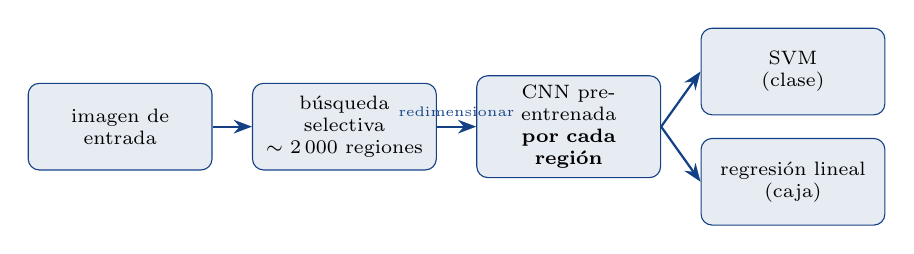
\begin{tikzpicture}[
			node distance=0.5cm,
			stage/.style={draw=mitblue, fill=mitblue!10, rounded corners, font=\scriptsize, align=center, minimum height=1.1cm, text width=2.1cm},
			arr/.style={-{Stealth}, thick, mitblue}]
			\node[stage] (img) {imagen de entrada};
			\node[stage, right=of img] (ss) {búsqueda selectiva\\$\sim 2\,000$ regiones};
			\node[stage, right=of ss] (cnn) {CNN pre-entrenada\\\textbf{por cada región}};
			\node[stage, right=of cnn, yshift=0.7cm] (svm) {SVM\\(clase)};
			\node[stage, right=of cnn, yshift=-0.7cm] (reg) {regresión lineal\\(caja)};
			\draw[arr] (img) -- (ss);
			\draw[arr] (ss) -- node[above, font=\tiny] {redimensionar} (cnn);
			\draw[arr] (cnn.east) -- (svm.west);
			\draw[arr] (cnn.east) -- (reg.west);
		\end{tikzpicture}
	\end{center}
	\begin{enumerate}
		\item \textbf{Búsqueda selectiva} extrae propuestas de región de varios tamaños, cada una etiquetada con una clase y una caja real.
		\item Cada propuesta se redimensiona y pasa por una CNN pre-entrenada truncada antes de la capa de salida.
		\item Con las características de cada región se entrenan \textbf{SVMs} (una por clase) para clasificar.
		\item Una \textbf{regresión lineal} ajusta la caja.
	\end{enumerate}
	\begin{alertblock}{Limitación}
		Miles de pasadas \textbf{independientes} de la CNN por imagen: demasiado lento para aplicaciones reales.
	\end{alertblock}
\end{frame}

\begin{frame}{Fast R-CNN (Girshick, 2015)}
	\textbf{Idea:} calcular la CNN una sola vez sobre la \textbf{imagen completa} y recortar las regiones sobre el mapa de características.
	\begin{center}
		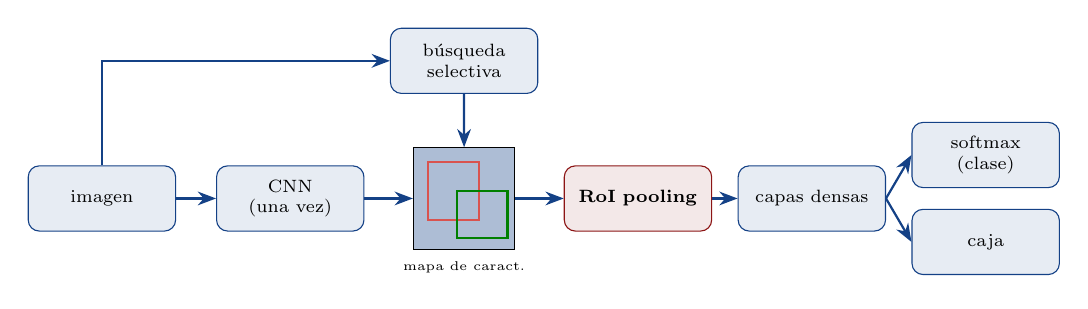
\begin{tikzpicture}[scale=0.92, every node/.style={transform shape},
			stage/.style={draw=mitblue, fill=mitblue!10, rounded corners, font=\scriptsize, align=center, minimum height=0.9cm, text width=1.8cm},
			arr/.style={-{Stealth}, thick, mitblue}]
			\node[stage] (img) at (0,0) {imagen};
			\node[stage] (cnn) at (2.6,0) {CNN\\(una vez)};
			\node[draw=black, fill=mitblue, fill opacity=0.35, minimum width=1.4cm, minimum height=1.4cm] (fm) at (5,0) {};
			\draw[bboxred, thick] (4.5,-0.3) rectangle (5.2,0.5);
			\draw[bboxgreen, thick] (4.9,-0.55) rectangle (5.6,0.1);
			\node[font=\tiny, below=1pt] at (fm.south) {mapa de caract.};
			\node[stage] (ss) at (5,1.9) {búsqueda selectiva};
			\node[stage, fill=StanfordRed!10, draw=StanfordRed] (roi) at (7.4,0) {\textbf{RoI pooling}};
			\node[stage] (fc) at (9.8,0) {capas densas};
			\node[stage] (cls) at (12.2,0.6) {softmax (clase)};
			\node[stage] (box) at (12.2,-0.6) {caja};
			\draw[arr] (img) -- (cnn);
			\draw[arr] (cnn) -- (fm);
			\draw[arr] (img.north) |- (ss.west);
			\draw[arr] (ss) -- (fm);
			\draw[arr] (fm) -- (roi);
			\draw[arr] (roi) -- (fc);
			\draw[arr] (fc.east) -- (cls.west);
			\draw[arr] (fc.east) -- (box.west);
		\end{tikzpicture}
	\end{center}
	\begin{itemize}
		\item Entrada $1\times c\times h_1\times w_1$ $\rightarrow$ la CNN produce un mapa $1\times c\times h_2\times w_2$.
		\item Las $n$ propuestas tienen tamaños distintos; \textbf{RoI pooling} convierte cada una en un tensor de forma fija $h_2\times w_2$ $\Rightarrow$ salida $n\times c\times h_2\times w_2$.
		\item Capas densas comunes predicen \textbf{clase} ($n\times q$) y \textbf{caja} ($n\times 4$).
	\end{itemize}
\end{frame}

\begin{frame}{RoI Pooling}
	\begin{columns}[c]
		\begin{column}{0.48\textwidth}
			A diferencia del pooling usual, aquí se fija el tamaño de la \textbf{salida} $h_2\times w_2$:
			\begin{itemize}
				\item La región de $h\times w$ se divide en una grilla de $h_2\times w_2$ subventanas de tamaño aproximado $\frac{h}{h_2}\times\frac{w}{w_2}$.
				\item De cada subventana se toma el \textbf{máximo}.
			\end{itemize}
			\vspace{0.2cm}
			\textbf{Ejemplo:} mapa $4\times4$, región $3\times3$ superior izquierda, salida $2\times2$:
			\begin{align*}
				\max(0,1,4,5)&=5, & \max(2,6)&=6,\\
				\max(8,9)&=9, & \max(10)&=10.
			\end{align*}
		\end{column}
		\begin{column}{0.5\textwidth}
			\begin{center}
				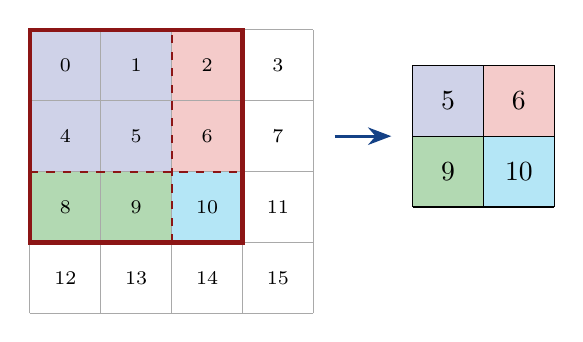
\begin{tikzpicture}[scale=0.9]
					% subventanas
					\fill[bboxblue!30] (0,2) rectangle (2,4);
					\fill[bboxred!30] (2,2) rectangle (3,4);
					\fill[bboxgreen!30] (0,1) rectangle (2,2);
					\fill[UCMBlue!30] (2,1) rectangle (3,2);
					\draw[mitgray] (0,0) grid (4,4);
					\foreach \y in {0,...,3}\foreach \x in {0,...,3}{
						\pgfmathtruncatemacro\v{\x+4*\y}
						\node[font=\scriptsize] at (\x+0.5,3.5-\y) {\v};
					}
					\draw[StanfordRed, ultra thick] (0,1) rectangle (3,4);
					\draw[StanfordRed, thick, dashed] (2,1) -- (2,4);
					\draw[StanfordRed, thick, dashed] (0,2) -- (3,2);
					\draw[-{Stealth}, very thick, mitblue] (4.3,2.5) -- (5.1,2.5);
					% salida
					\begin{scope}[xshift=5.4cm, yshift=1.5cm]
						\fill[bboxblue!30] (0,1) rectangle (1,2);
						\fill[bboxred!30] (1,1) rectangle (2,2);
						\fill[bboxgreen!30] (0,0) rectangle (1,1);
						\fill[UCMBlue!30] (1,0) rectangle (2,1);
						\draw (0,0) grid (2,2);
						\node at (0.5,1.5) {5}; \node at (1.5,1.5) {6};
						\node at (0.5,0.5) {9}; \node at (1.5,0.5) {10};
					\end{scope}
				\end{tikzpicture}
			\end{center}
		\end{column}
	\end{columns}
\end{frame}

\begin{frame}{Faster R-CNN (Ren et al., 2015)}
	\textbf{Idea:} reemplazar la búsqueda selectiva por una \textbf{red de propuestas de región} (RPN) que se entrena junto al detector.
	\vspace{-0.2cm}
	\begin{columns}[T]
		\begin{column}{0.55\textwidth}
			\begin{block}{Red de Propuestas de Región (RPN)}
				\begin{enumerate}
					\item Convolución $3\times3$ (padding 1) sobre el mapa de la CNN: un vector de $c$ características por celda.
					\item Centrar en cada celda \textbf{anclas} de varias escalas y razones.
					\item Para cada ancla, predecir \textbf{objeto/fondo} (clasificación binaria) y su \textbf{desplazamiento}.
					\item Aplicar \textbf{NMS} a las cajas predichas como objeto: éstas son las propuestas para RoI pooling.
				\end{enumerate}
			\end{block}
		\end{column}
		\begin{column}{0.43\textwidth}
			\begin{center}
				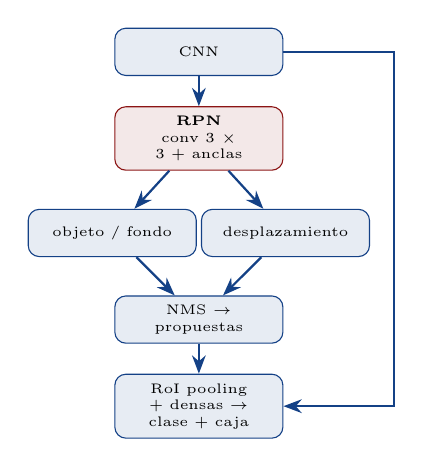
\begin{tikzpicture}[
					stage/.style={draw=mitblue, fill=mitblue!10, rounded corners, font=\tiny, align=center, minimum height=0.6cm, text width=1.9cm},
					arr/.style={-{Stealth}, thick, mitblue}]
					\node[stage] (cnn) at (0,0) {CNN};
					\node[stage, fill=StanfordRed!10, draw=StanfordRed] (rpn) at (0,-1.1) {\textbf{RPN}\\conv $3\times3$ + anclas};
					\node[stage] (bin) at (-1.1,-2.3) {objeto / fondo};
					\node[stage] (off) at (1.1,-2.3) {desplazamiento};
					\node[stage] (nms) at (0,-3.4) {NMS $\rightarrow$ propuestas};
					\node[stage] (roi) at (0,-4.5) {RoI pooling + densas $\rightarrow$ clase + caja};
					\draw[arr] (cnn) -- (rpn);
					\draw[arr] (rpn) -- (bin);
					\draw[arr] (rpn) -- (off);
					\draw[arr] (bin) -- (nms);
					\draw[arr] (off) -- (nms);
					\draw[arr] (nms) -- (roi);
					\draw[arr] (cnn.east) -- ++(1.4,0) |- (roi.east);
				\end{tikzpicture}
			\end{center}
		\end{column}
	\end{columns}
	\vspace{0.1cm}
	\small Entrenamiento \textbf{extremo a extremo} con 4 pérdidas (clase y caja del detector; objeto/fondo y caja de la RPN). Propuestas aprendidas $\Rightarrow$ bastan \textbf{menos} sin perder precisión.
\end{frame}

\begin{frame}{Mask R-CNN (He et al., 2017)}
	Si además se dispone de la posición de cada objeto \textbf{a nivel de píxel}, Faster R-CNN se extiende a \textbf{segmentación de instancias}.
	\begin{columns}[c]
		\begin{column}{0.55\textwidth}
			\begin{block}{RoI Align en lugar de RoI Pooling}
				RoI pooling \textbf{redondea} los bordes de la región y de las subventanas a la grilla del mapa, perdiendo precisión espacial. RoI Align mantiene las coordenadas reales y obtiene los valores por \textbf{interpolación bilineal}.
			\end{block}
			\begin{block}{Rama de máscaras}
				Una red totalmente convolucional (FCN) predice, para cada región, una \textbf{máscara binaria} del objeto, además de la clase y la caja.
			\end{block}
		\end{column}
		\begin{column}{0.43\textwidth}
			\begin{center}
				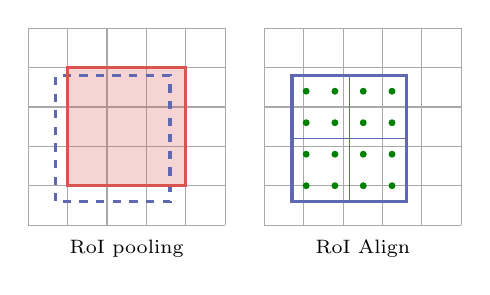
\begin{tikzpicture}[scale=0.5]
					\begin{scope}
						\draw[mitgray] (0,0) grid (5,5);
						\fill[bboxred, opacity=0.25] (1,1) rectangle (4,4);
						\draw[bboxblue, very thick, dashed] (0.7,0.6) rectangle (3.6,3.8);
						\draw[bboxred, very thick] (1,1) rectangle (4,4);
						\node[font=\scriptsize] at (2.5,-0.6) {RoI pooling};
					\end{scope}
					\begin{scope}[xshift=6cm]
						\draw[mitgray] (0,0) grid (5,5);
						\draw[bboxblue, very thick] (0.7,0.6) rectangle (3.6,3.8);
						\draw[bboxblue, thin] (2.15,0.6) -- (2.15,3.8);
						\draw[bboxblue, thin] (0.7,2.2) -- (3.6,2.2);
						\foreach \x in {1.06,1.79,2.51,3.24}\foreach \y in {1.0,1.8,2.6,3.4}{\fill[bboxgreen] (\x,\y) circle (2.5pt);}
						\node[font=\scriptsize] at (2.5,-0.6) {RoI Align};
					\end{scope}
				\end{tikzpicture}

				\scriptsize \textcolor{bboxblue}{región real}, \textcolor{bboxred}{región cuantizada}, \textcolor{bboxgreen}{puntos interpolados}.
			\end{center}
		\end{column}
	\end{columns}
\end{frame}

\begin{frame}{Comparación de Detectores}
	\begin{center}
		\footnotesize
		\begin{tabular}{llll}
			\toprule
			\textbf{Modelo} & \textbf{Propuestas} & \textbf{Aporte principal} & \textbf{Costo} \\
			\midrule
			R-CNN (2014) & búsqueda selectiva & CNN pre-entrenada por región & una CNN por región \\
			Fast R-CNN (2015) & búsqueda selectiva & CNN compartida + RoI pooling & una CNN por imagen \\
			Faster R-CNN (2015) & RPN (aprendida) & propuestas con anclas & extremo a extremo \\
			Mask R-CNN (2017) & RPN (aprendida) & RoI Align + rama FCN & + máscaras \\
			\midrule
			SSD (2016) & ninguna (anclas fijas) & predicción multiescala & una sola pasada \\
			\bottomrule
		\end{tabular}
	\end{center}
	\vspace{0.3cm}
	\begin{itemize}
		\item La evolución de R-CNN consiste en \textbf{eliminar cómputo redundante} y \textbf{reemplazar componentes hechos a mano} por módulos aprendidos.
		\item Los detectores de dos etapas suelen ser más precisos; los de una etapa, más rápidos.
	\end{itemize}
\end{frame}

% --- RESUMEN ---
\begin{frame}{Conclusiones}
	\begin{itemize}
		\item La detección de objetos predice, para un número variable de objetos, su \textbf{clase} y su \textbf{caja delimitadora}.
		\item Las \textbf{cajas ancla} discretizan el espacio de cajas posibles; cada ancla se etiqueta con una clase (o fondo) y un \textbf{desplazamiento} hacia la caja real según el \textbf{IoU}.
		\item En predicción, la \textbf{supresión de no-máximos} elimina las detecciones redundantes.
		\item Usar anclas sobre mapas de características de \textbf{varias escalas} permite detectar objetos de distintos tamaños con un número manejable de anclas.
		\item \textbf{SSD}: una etapa, predicción convolucional de clase y caja en cada escala; pérdida = entropía cruzada + $L_1$ enmascarada.
		\item \textbf{R-CNN} $\rightarrow$ \textbf{Fast} (RoI pooling) $\rightarrow$ \textbf{Faster} (RPN) $\rightarrow$ \textbf{Mask} (RoI Align + máscaras).
	\end{itemize}
\end{frame}

\begin{frame}{Referencias}
	\small
	\begin{itemize}
		\item A. Zhang, Z. C. Lipton, M. Li, A. J. Smola. \textit{Dive into Deep Learning}, cap. 14 ``Computer Vision'', secciones 14.3--14.8. \texttt{https://d2l.ai}
		\item R. Girshick, J. Donahue, T. Darrell, J. Malik. Rich feature hierarchies for accurate object detection and semantic segmentation. \textit{CVPR}, 2014.
		\item R. Girshick. Fast R-CNN. \textit{ICCV}, 2015.
		\item S. Ren, K. He, R. Girshick, J. Sun. Faster R-CNN: Towards real-time object detection with region proposal networks. \textit{NeurIPS}, 2015.
		\item W. Liu et al. SSD: Single shot multibox detector. \textit{ECCV}, 2016.
		\item K. He, G. Gkioxari, P. Dollár, R. Girshick. Mask R-CNN. \textit{ICCV}, 2017.
	\end{itemize}
\end{frame}

\end{document}
